% #############################################################################
% This is Chapter 2
% !TEX root = ../main.tex
% #############################################################################
% Change the Name of the Chapter i the following line
\fancychapter{Background}\label{chap:back}
% The following line allows to ref this chapter

This chapter introduces the fundamental concepts of \glsxtrfull{IR}, while \glsxtrfull{NLP} will be covered in the next chapter, which covers state-of-the-art. \gls{IR} has evolved from lexical to semantic search, and understanding these approaches is essential to contextualize how \gls{NLP} subsequently enables agents to reason over retrieved information to provide more intelligent responses. The following section presents these \gls{IR} approaches and the optimizations that derived from them.
\section{Background on Transformers} 
\label{sec:transformer}
\subsection{The Transition from Sequential to Attention-Based Models}  
Traditional sequence transduction models, such as \glsxtrfullpl{RNN} and its variants (e.g., \glsxtrfull{LSTM} \cite{hochreiter1997lstm} and \glsxtrfull{GRU} \cite{cho2014gru}), were widely used in tasks such as machine translation and language modeling. Although effective, these models relied on sequential calculations, which limited parallelization and computational efficiency, particularly in long sequences \cite{vaswani2017attention}.

In 2017, Vaswani et al. introduced the Transformer architecture, marking a paradigm shift from these sequential models. Transformer relies exclusively on attention mechanisms, specifically self-attention, to model dependencies between input and output sequences. By removing recursive and convolutional operations, Transformer achieves faster training times and superior performance in generative tasks \cite{vaswani2017attention}.

\begin{figure}[H]
    \centering
    % First image
    \centering
    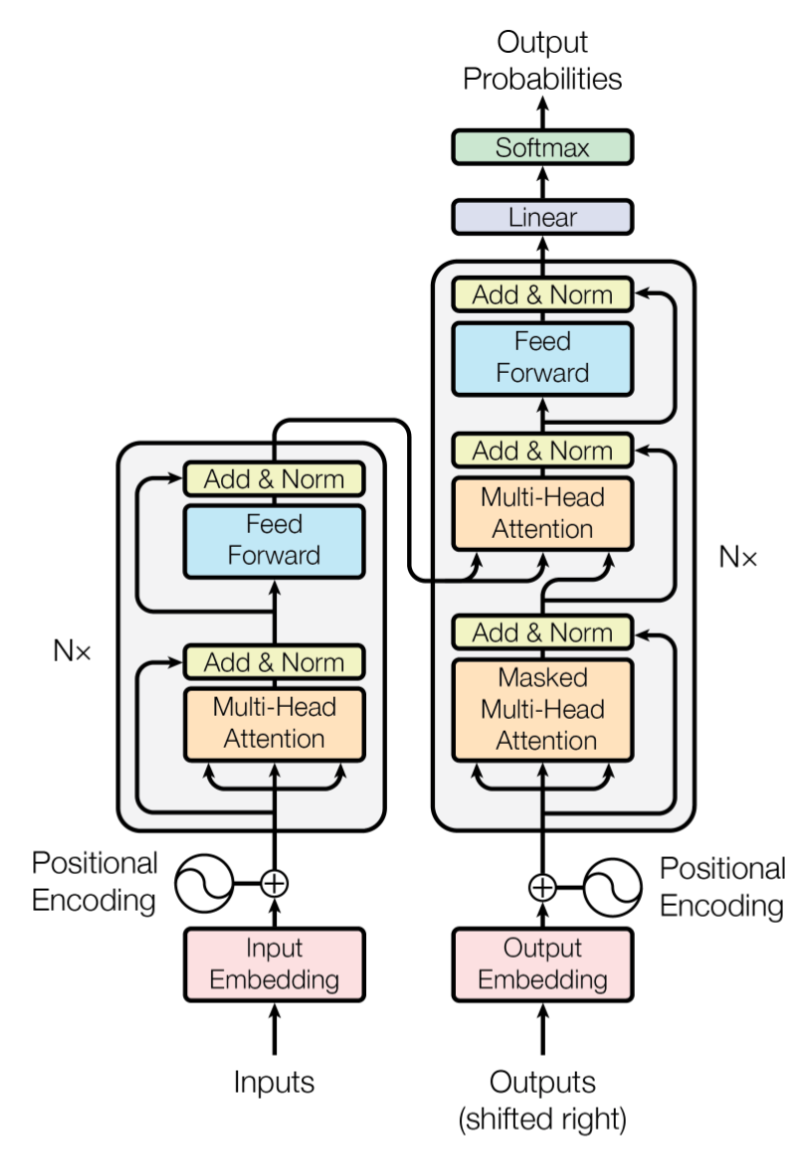
\includegraphics[width=0.45\linewidth]{Images/Transformer_architecture3.png}
    \caption{Transformer Architecture from~\cite{vaswani2017attention}}\label{fig:Tranformer}
\end{figure}

The Transformer is fundamentally structured as an \textit{encoder-decoder} model. The \textbf{encoder} processes the input sequence and produces a continuous vector representation, while the \textbf{decoder} generates the output sequence one token at a time, conditioning on both the encoder output and previously generated tokens. This architecture allows the model to handle input and output sequences at variable length and is the foundation for tasks such as machine translation, summarization, and question answering.

\subsection{Main Innovations in Transformer Architecture}  
\begin{itemize}
    \item \textbf{Embeddings}: Learned embeddings convert input and output tokens to vectors of dimension $d$ depending on the dimension of the model. Tokens are discrete symbols of words or subwords.
    \item \textbf{Positional Coding}:  
    Transformers do not need recurrence nor convolution, instead some information about relative or absolute position of the tokens is injected in the sequences. These are the positional encodings added to the input embeddings \cite{vaswani2017attention}.
    \item \textbf{Layer Normalization}: Applied after attention and feed-forward layers (or before, in pre-norm variants), layer normalization stabilizes training by normalizing activations to zero mean and unit variance. It is essential for enabling deep stacking of transformer blocks without training instability.
    
    \item  \textbf{Scaled Dot-Product Attention} \ref{eq:Attention}: Is an attention function \ref{eq:Attention} that maps a query and a set of key-value pairs to an output.
    \begin{equation}
        \label{eq:Attention}
        \text{Attention}(Q,K,V) = softmax(\frac{QK^T}{\sqrt{d_k}})V 
    \end{equation}
    The scaling factor $\sqrt{d_k}$ prevents gradient vanishing in attention weights: without it, large dot products would lead to very small gradients after softmax. This stabilizes training and allows for better gradient flow during backpropagation.
    \begin{itemize}
        \item Q is a set of queries packed together into a matrix.
        \item K and V are also matrices packed together of keys and values, respectively
    \end{itemize}
    \item \textbf{Multi-Head Attention}:  Queries, keys and values are linearly projected $h$ different times with different learned linear projections \ref{eq:MultiHead}. Multiple attention heads allow the model to jointly attend to information from different representation subspaces at different positions, enabling simultaneous focus on syntactic and semantic features. This is more effective than a single large attention head.
    \begin{equation}
        \label{eq:MultiHead}
        \text{MultiHead}(Q,K,V) = \text{Concat}(head_1, ..., head_h)W^O  
    \end{equation}
    \begin{itemize}
        \item $head_i = \text{Attention}(QW_i^Q, KW_i^K,VW_i^V)$
    \end{itemize}
    
    \item \textbf{Residual Connections}: Skip connections are placed around both the attention and feed-forward sub-layers, allowing gradients to flow directly through the network. This is critical for training very deep models, as it mitigates the vanishing gradient problem and enables stable learning of identity mappings.

    \item \textbf{Feed-Forward}:  A Position-Wise Feed-Forward Network (FFN) \ref{eq:FNN} is a fully connected neural network designed to independently process each position in the sequence.  While FNN \ref{eq:FNN} operates identically at all positions, the parameters vary between layers. The dimension of the inner-layer has a larger dimension than the model's dimension to increase its capacity to learn complex transformations~\cite{vaswani2017attention}.
    \begin{equation}
        \label{eq:FNN}
        \text{FNN}(x) = \max(0,xW_1+b_1)W_2+b_2
    \end{equation}
\end{itemize}

\subsection{Self-Attention vs. Cross-Attention}
While the attention mechanism described above is \textit{self-attention}—where queries, keys, and values all come from the same sequence—the Transformer decoder also employs \textit{cross-attention}. In cross-attention, queries come from the decoder's previous layer, while keys and values come from the encoder output. This allows the decoder to attend to relevant encoder representations when generating each output token, forming the crucial bridge between encoded input and generated output in tasks like machine translation.

\subsection{Connection to Modern Language Models}  
The Transformer architecture achieved top results in machine translation tasks, such as on the WMT 2014 English-German and English-French datasets, with significantly shorter training times compared to previous models that relied on recurrent architectures. For example, the model achieved a BLEU score of 28.4 on English-to-German translation, outperforming previous architectures by more than 2 BLEU points \cite{vaswani2017attention}.

While the original Transformer used both encoder and decoder, subsequent adaptations have proven remarkably versatile: \textit{encoder-only} models like \gls{BERT} leverage masked self-attention for deep bidirectional understanding, while \textit{decoder-only} models like \gls{GPT} stack self-attention layers to autoregressively generate text one token at a time. These architectural variants, combined with massive pretraining on diverse text corpora, form the foundation of modern \glsxtrfullpl{LLM}. The Transformer's core principles of self-attention and scalability have thus enabled the current era of large language models.

\section{\glsxtrfull{LLM}}
\label{sec:llm}
Building on the Transformer architectures described in Section~\ref{sec:transformer}, modern \glsxtrfullpl{LLM} like \gls{BERT} and \gls{GPT} have become the foundation for advanced \glsxtrfull{NLP} tasks. Summarization and reasoning are key capabilities of \glsxtrfull{AAI} systems, which must distill context, interpret complex instructions, and generate coherent responses. This section focuses on the practical choice of \gls{LLM} provider for this thesis.

While open-source models such as LLaMA, Mistral, Falcon, and Qwen2.5 (available via Hugging Face or ollama) provide valuable baseline options, this thesis primarily relies on the OpenAI API. Compared to hosting open-source models on local servers, OpenAI's approach is cheaper, higher-performing, and more scalable, since it removes infrastructure costs while providing access to cutting-edge systems like \gls{GPT}-4o and \gls{GPT}-4o-mini.

Strong empirical evidence supports the OpenAI choice, even for Portuguese language tasks:
\begin{itemize}
  \item On the Brazilian ENEM entrance exam, \gls{GPT}-4 with Chain-of-Thought prompting achieved 87\% accuracy, surpassing \gls{GPT}-3.5 by 11 points \cite{arxiv2303.17003}.
  \item On the Portuguese National Medical Residency Access Examination, \gls{GPT}-4o outperformed LLaMA 3.1 by 7–11\% across medical domains \cite{pmc12166901}.
\end{itemize}

Given these performance advantages, even performing well in the Portuguese language, along with cost-effectiveness and scalability, OpenAI \glspl{LLM} are adopted in this thesis as the principal agents for reasoning and summarization.


\section{\glsxtrfull{RAG}}
\label{sec:rag}

(\glsxtrfull{RAG}) is a framework designed to improve performance on knowledge-intensive \gls{NLP} tasks. It combines \textit{parametric knowledge}, implicitly stored in the parameters of a pre-trained \glsxtrfull{LLM}, with \textit{non-parametric knowledge}, retrieved from external sources such as document collections or databases. Traditional \glsxtrfullpl{LLM} encode knowledge implicitly in their parameters, which is static, cannot be updated without retraining, and may become outdated. \gls{RAG} mitigates this limitation by introducing a retrieval component that accesses external, explicit, and up-to-date information. Instead of relying solely on the static internal knowledge of the model, RAG enhances generation with dynamically retrieved and contextually relevant information.

\subsection{RAG Pipeline Architecture}
A typical RAG pipeline operates in three sequential stages: (1) \textbf{Retrieval}, where the system searches an external knowledge base (e.g., a vector database) to retrieve the most relevant documents or passages given an input query; (2) \textbf{Augmentation}, where the retrieved documents/chunks of text are then combined with the query to form an enriched prompt, providing the \gls{LLM} with additional context; and (3) \textbf{Generation}, where the \gls{LLM} conditions its output on both the query and the retrieved context, producing responses from known sources. To use AI for semantic search effectively, it is essential to use \gls{RAG} to ensure access to up-to-date information.

\subsection{Retrieval Methods in RAG}

The retrieval stage can be implemented in multiple ways, ranging from traditional sparse methods to modern dense retrieval techniques. This subsection covers both approaches.

\subsubsection{Sparse Retrieval Methods}

Traditional sparse retrieval approaches rely on \textbf{sparse representations}, where documents are represented as bags of words or weighted keyword vectors. These are sparse vector space models that match keywords efficiently via an inverted index, representing both queries and documents as high-dimensional, sparse vectors with term-based weighting. While these models are often effective for keyword-based matches, they struggle when queries and relevant documents use synonyms or paraphrases that do not share surface-level terms.

Well-known sparse retrieval methods include TF-IDF and BM25, which are detailed below.

\paragraph{TF-IDF (Term Frequency-Inverse Document Frequency)}

TF-IDF is a foundational term-weighting and ranking scheme in information retrieval systems \cite{tf-idf}. Its primary purpose is to measure how important a term is to a particular document within a large collection of documents. While frequency counts can highlight terms that often appear, they do not account for how common or rare those terms are across the entire dataset. TF-IDF addresses this by diminishing the weight of terms that occur frequently across many documents and increasing the weight of terms that appear in fewer documents (more distinctive terms).

The \glsxtrfull{TF} measures how often a term \textit{t} appears in a single document \textit{d}:
\begin{equation}
    \label{eq:tf} 
    \text{TF}(t,d)=f_{t,d}
\end{equation}
where $f_{t,d}$ is the frequency of term $t$ in document $d$.

For longer documents, a normalization is applied:
\begin{equation}
    \label{eq:tf(t,d)}
    \text{TF}(t,d) = \frac{f_{t,d}}{\sum_{t'}f_{t',d}}
\end{equation}

The inverse document frequency (IDF) measures how common a term is across the entire collection of documents. If a term appears in many documents, it is less useful for distinguishing those documents. A higher IDF means a term appears in fewer documents, indicating its uniqueness. Let \textit{N} be the total number of documents in the collection, and $n_t$ be the number of documents in which the term appears. \textit{IDF} is defined as:
\begin{equation}
    \label{eq:idftf}
    \text{IDF}(t)=\log\frac{N}{n_t}
\end{equation}

TF-IDF is then the combination of both TF and IDF:
\begin{equation}
    \label{eq:tfidf}
    \text{TF-IDF}(t,d) = f_{t,d} \times \log\left(\frac{N}{n_t}\right)
\end{equation}

The uniqueness of the TF-IDF approach in retrieval is how it combines a local component (frequency in the current document) and a global component (frequency across the entire collection). TF-IDF has the advantage of being straightforward, interpretable, and computationally efficient.
\paragraph{BM25 (Okapi BM25)}

The Okapi BM25 system, first introduced in \cite{Bm25foundation}, culminated in BM25 (short for ``Best Match 25''), a probabilistic information retrieval model. BM25 improves upon TF-IDF by using a probabilistic basis rather than a purely heuristic one, and by introducing parameters to control term frequency saturation and document length normalization.

The BM25 formula is similar to TF-IDF in structure, but uses a more sophisticated formulation of the IDF component that is more stable and empirically effective. The IDF component per term \textit{t} is computed as:
\begin{equation}
    \label{eq:idfbm25}
    \text{IDF}(t) = \log \frac{N-n_t+0.5}{n_t+0.5}
\end{equation}
where N is the total number of documents in the collection and $n_t$ is the number of documents containing term \textit{t}.

The BM25 formula to score a document $d$ given a query $q$ (consisting of multiple terms) is:
\begin{equation}
    \label{eq:bm25}
    \textit{BM25}(d,q) = \sum_{t \in q} \text{IDF}(t) \cdot \frac{(k_1+1)\cdot f_{t,d}}{f_{t,d}+k_1(1-b+b \cdot \frac{|d|}{avgdl})}
\end{equation}
where:
\begin{itemize}
\item $d$ is a given document.
\item $q$ a user's query, consisting of terms.
\item $|d|$ is the length of a document in terms of the number of tokens.
\item $avgdl$ is average document length across the entire collection.
\item $k_1$ and $b$ are tuning parameters:
\begin{itemize}
    \item $k_1$ controls the saturation of \glsxtrfull{TF}, by preventing over-emphasis on very frequent terms.
    \item $b$ controls document length normalization. If $b = 1$, the normalization is directly proportional to how much longer (or shorter) the document ($|d|$) is compared to average document length ($avgdl$). If $b=0$, no document length normalization is applied.
\end{itemize}
\end{itemize}

\subsubsection{Dense Retrieval Methods}

Recent advancements in \gls{LLM}, particularly transformer-based models like \gls{BERT} \cite{bertpretrainingdeepbidirectional}, have led to dense retrieval systems that overcome the limitations of sparse methods. In dense retrieval, queries and documents are represented as low-dimensional vectors that better capture semantic similarity. However, dense methods often require large training datasets (i.e., labeled question–passage pairs) to surpass classical methods such as TF-IDF/BM25. Modern pre-trained language models help mitigate this requirement by providing robust initial embeddings that can be fine-tuned on relatively smaller sets of question–context examples, enabling dense retrieval methods to outperform traditional sparse approaches in many open-domain QA tasks.
\paragraph{Dense Passage Retrieval (DPR)}
\label{par:dpr}

Dense Passage Retrieval (DPR), introduced by Karpukhin et al.~\cite{densepassageretrievalopendomainkarpukhin2020}, is a \textit{dense retrieval} method designed specifically for \textit{open-domain question answering}. Unlike conventional approaches that rely on \textit{purely lexical} matches (e.g., TF-IDF and BM25), DPR employs \gls{BERT}-based encoders to map questions and passages into a shared, dense embedding space, enabling \textit{semantic} rather than strictly \textit{keyword-based} retrieval. By leveraging modern \gls{LLM} such as \gls{BERT}~\cite{bertpretrainingdeepbidirectional} and LLaMA, which come with strong pre-trained representations, DPR can be fine-tuned with comparatively fewer labeled samples. This allows the system to capture semantic relationships between questions and passages, thereby mitigating the shortcomings of traditional methods that rely solely on term overlap.

The DPR architecture is based on a dual-encoder architecture~\cite{dualencoderarchitecture}. Specifically, in Karpukhin et al.'s formulation~\cite{densepassageretrievalopendomainkarpukhin2020}, both encoders are initialized from the same pre-trained \gls{BERT} model but are then fine-tuned separately for their respective tasks. A Question Encoder \(E_Q\) takes a question as input and produces a single vector embedding \(\mathbf{q_i}\), while a Passage Encoder \(E_P\) processes a passage to produce a single vector embedding \(\mathbf{p_j}\). Once encoded, each question and passage becomes a fixed-dimensional vector (e.g., 768 dimensions). To measure the similarity between a question \((\mathbf{q})\) and a passage \((\mathbf{p})\), the dot product of their embeddings is computed:
\begin{equation}
    \label{eq:dot_sim}
    \text{similarity}(\mathbf{q}, \mathbf{p}) = E_Q(\mathbf{q})^T \, E_P(\mathbf{p})
\end{equation}
where $\mathbf{q}$ is the question embedding and $\mathbf{p}$ is the passage embedding, both produced by their respective encoders.

\section{Sentence Transformers}
\label{sec:Sentence-Transformers}
Sentence Transformers are \gls{BERT}-based encoder models designed to generate dense vector representations (embeddings) of entire sentences or passages. 
They were introduced in 2019 \cite{reimers2019sentencebertsentenceembeddingsusing} as an adaptation of the \gls{BERT} architecture, which was originally built for token-level classification tasks.

With the use of Siamese and Triplet network structures on top of \gls{BERT}, SBERT modifies the architecture to operate at the sentence level. Instead of encoding a pair of sentences jointly, as in the cross-encoder setup of standard \gls{BERT}, SBERT processes each sentence independently with a shared \gls{BERT} encoder. This produces fixed-size embeddings that can later be compared directly using cosine similarity or other distance metrics, making large-scale similarity search computationally feasible.

In a Siamese setup, two identical \gls{BERT} encoders with shared weights process different input sentences. Their embeddings are then compared, allowing the network to learn similarity or classification objectives. This design ensures that semantically similar sentences are mapped to nearby points in the embedding space, while dissimilar ones are pushed apart.

Triplet networks extend this idea by processing three inputs simultaneously: an anchor sentence, a positive sentence with similar meaning, and a negative sentence with unrelated meaning. The model is trained to minimize the distance between the anchor and the positive embedding, while maximizing the distance between the anchor and the negative embedding. This objective directly enforces a semantically meaningful structure in the embedding space, making the representations more robust for tasks such as \glsxtrfull{STS} and information retrieval.
\begin{figure}[h!]
    \centering
    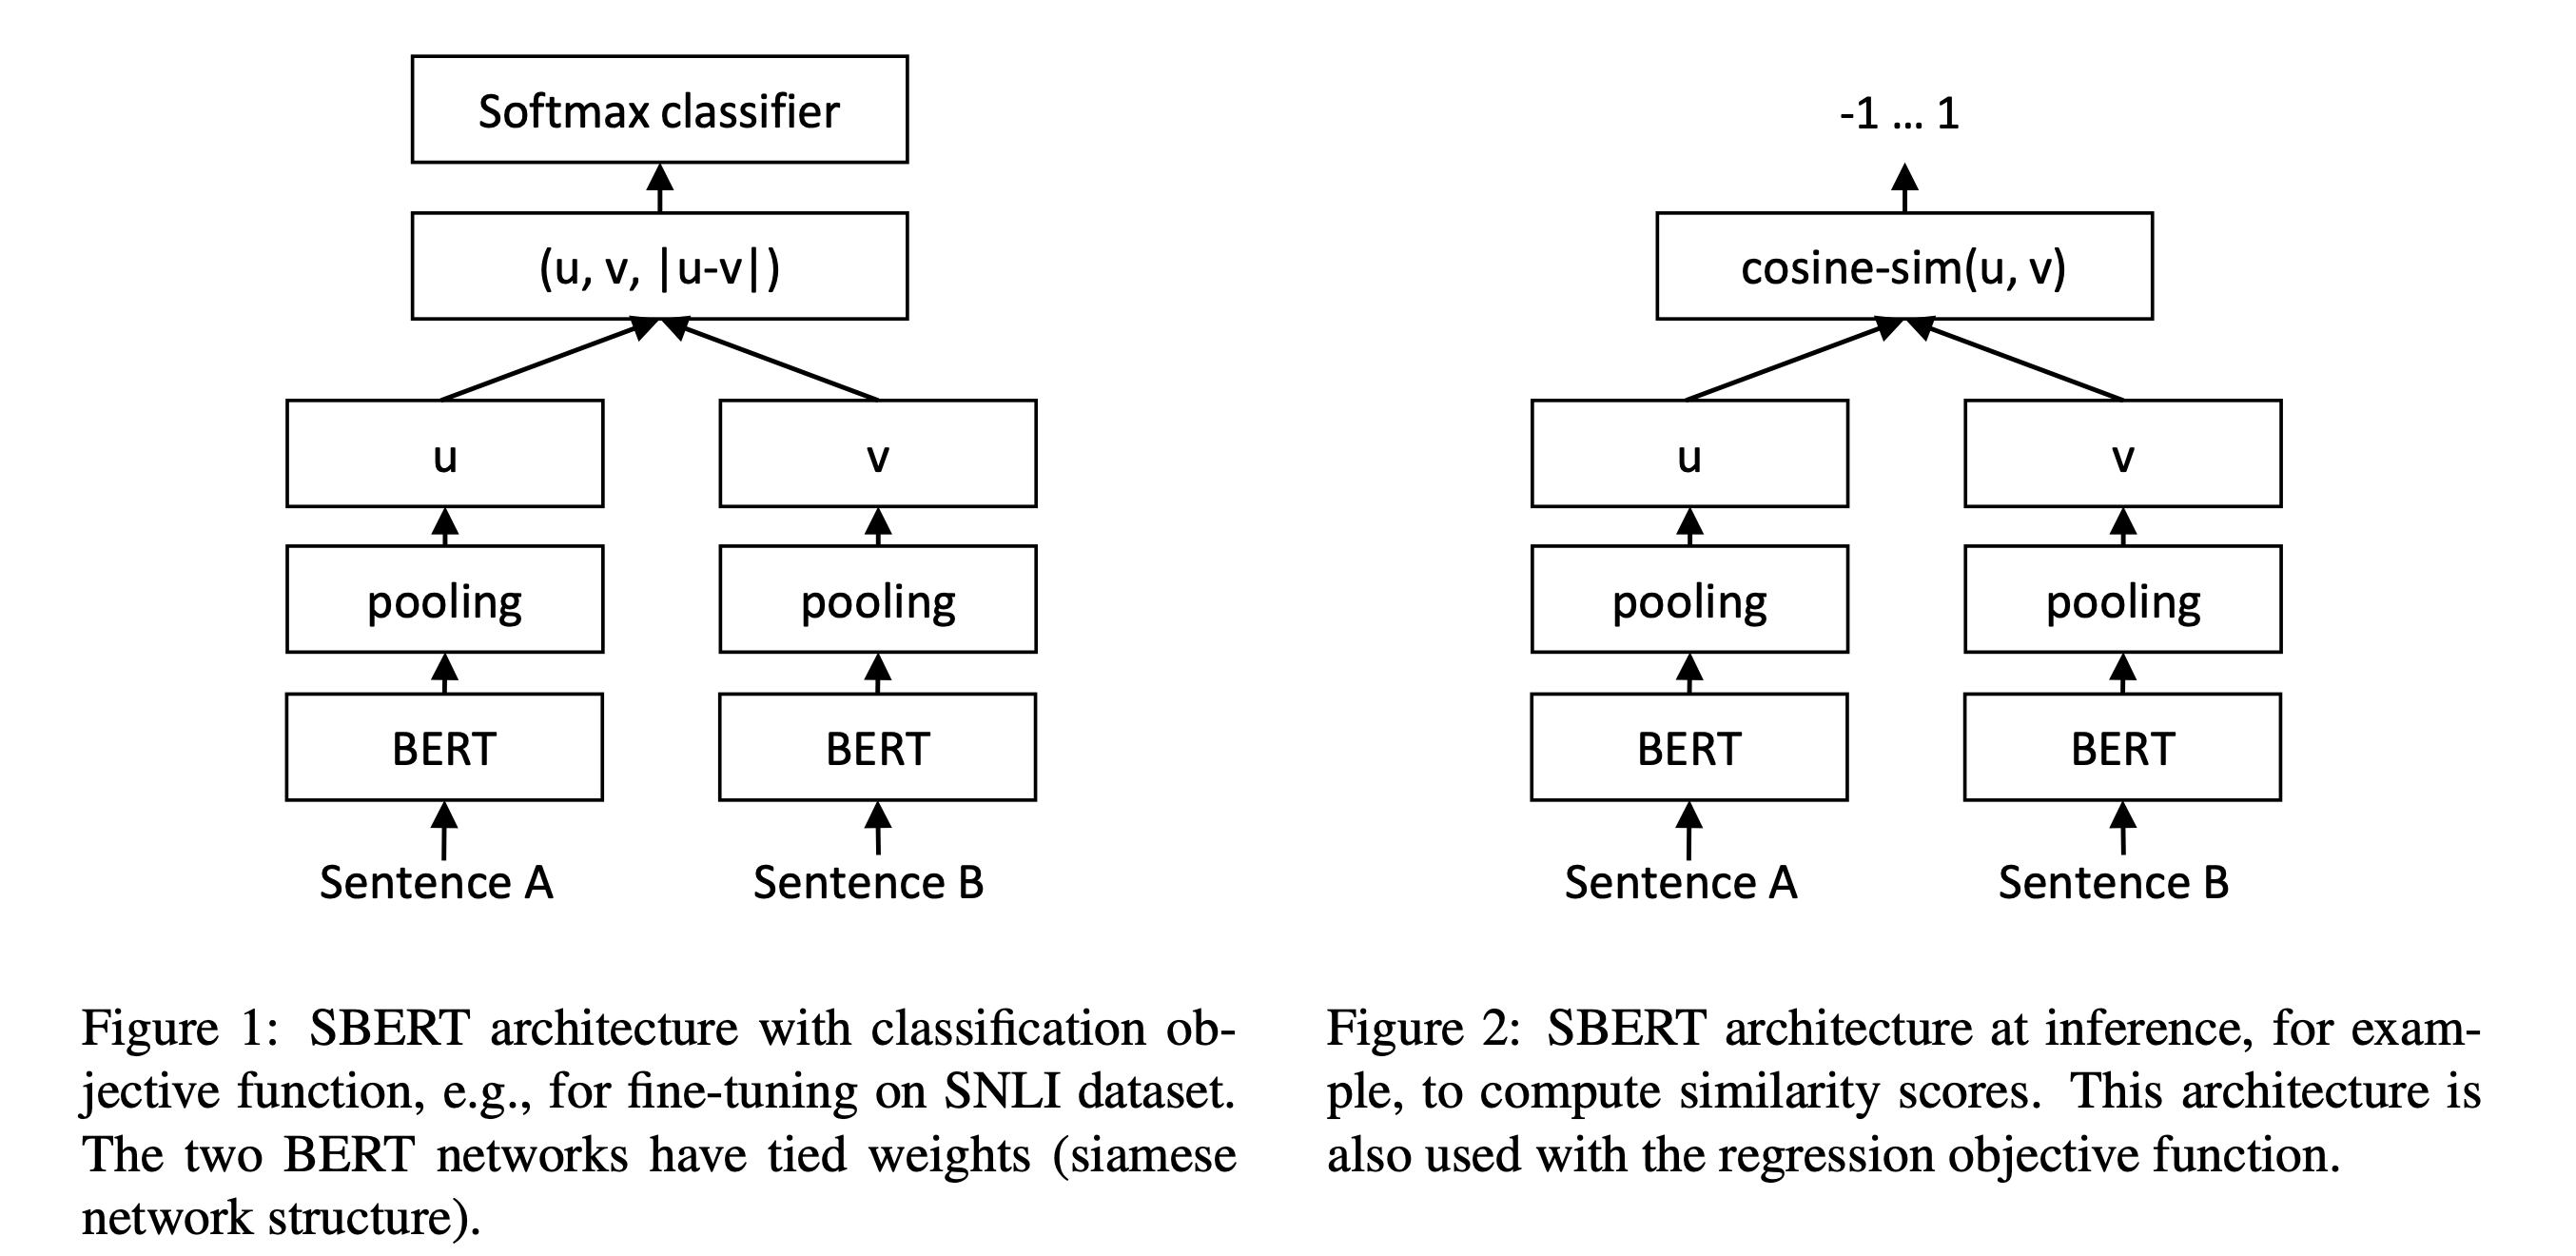
\includegraphics[width=1\linewidth]{Images/sentence_transformer.png}
    \caption{Sentence Transformer Architecture explained in~\cite{reimers2019sentencebertsentenceembeddingsusing}}
    \label{fig:sentence-transformer-architecture}
\end{figure}
Since \gls{BERT} outputs contextual embeddings for individual tokens, an additional pooling layer is required to derive a single sentence vector, as shown in Figure~\ref{fig:Sentence_embedding}. In \cite{reimers2019sentencebertsentenceembeddingsusing}, the preferred pooling method for \gls{STS} tasks is mean pooling, which turns multiple token embeddings into a single sentence embedding.\footnote{Other pooling strategies, such as using the \texttt{[CLS]} token or max pooling, were also evaluated but performed worse for semantic similarity tasks.}

\begin{figure}[h!]
    \centering
    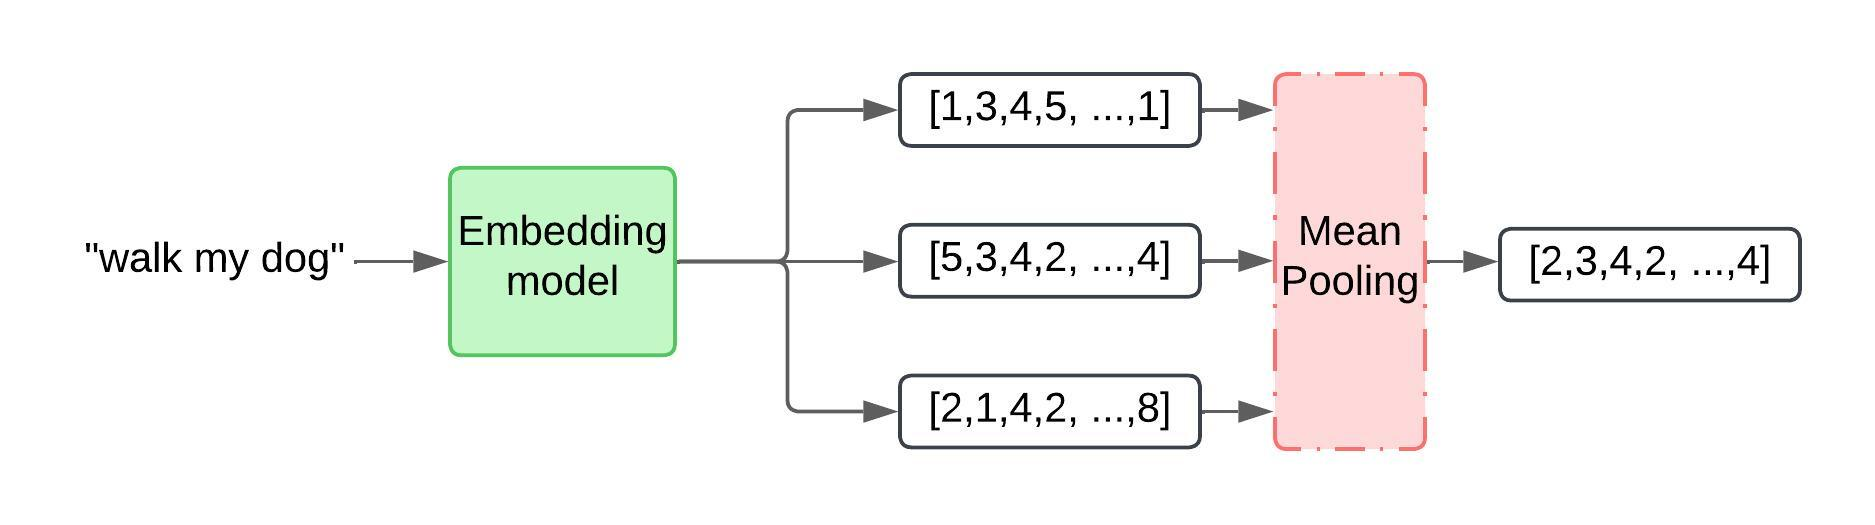
\includegraphics[width=1\linewidth]{Figures/Sentence_Embedding.jpeg}
    \caption{Example illustration of sentence embedding through mean pooling.}\label{fig:Sentence_embedding}
\end{figure}

To ensure that these embeddings capture sentence-level meaning, SBERT is fine-tuned on tasks such as (\gls{NLI}), (\gls{STS}), and triplet training. 

When trained on \gls{NLI} data with a classification objective, SBERT further compares pairs of sentence embeddings by constructing a combined feature vector $(u, v, |u-v|)$, where $u$ and $v$ are the pooled embeddings of the two sentences. This representation proved effective in downstream tasks such as the Semantic Textual Similarity benchmark (\gls{STS}-b).

The quality of a Sentence Transformer is ultimately reflected in the accuracy and robustness of the embeddings it produces. Recent research has extended these methods to Portuguese, with the current state-of-the-art being the \textit{Serafim 900M IR} model \cite{gomes2024opensentenceembeddingsportuguese}, which has been specifically trained and benchmarked for \gls{STS} and \gls{IR} tasks.

\section{Vector Databases}
\label{sec:vector-store}
As described in more detail Section~\ref{sec:Sentence-Transformers}, embedding models transform unstructured data (e.g., text, images, or audio) into high-dimensional numerical vectors that capture semantic relationships. In such a vector space, similar objects are positioned closer together, while unrelated ones are placed farther apart. For example, the terms \emph{dog} and \emph{wolf} would be embedded near each other, whereas \emph{banana} would appear in a distant region (see Fig.~\ref{fig:vector-embedding}).  

A vector database stores these embeddings and supports efficient similarity search through vector indexing techniques, enabling similarity search at scale.
\begin{figure}[h]
    \centering
    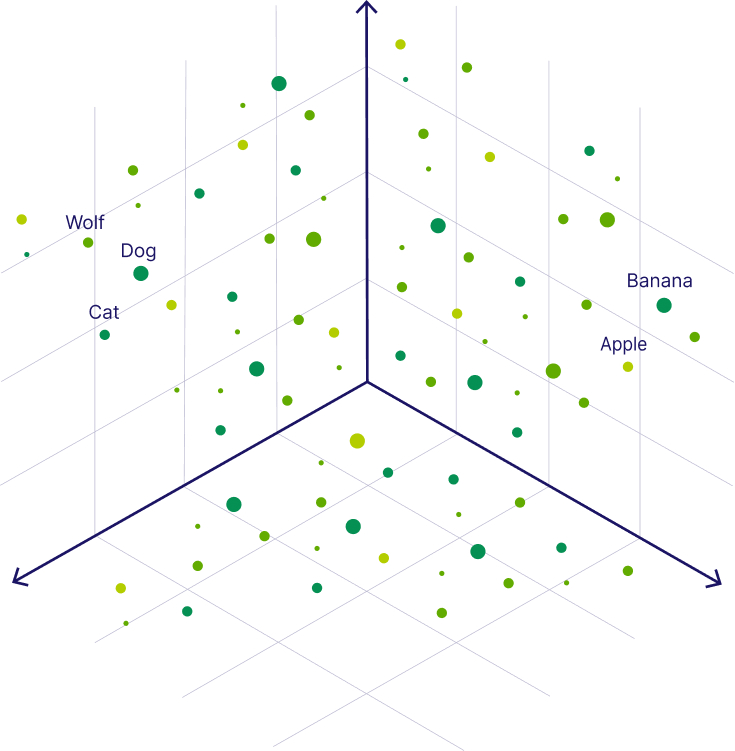
\includegraphics[width=0.55\linewidth]{Images/vector-embedding.jpg}
    \caption{Example of vector embeddings where semantically related terms are placed closer in the vector space \cite{weaviate}}
    \label{fig:vector-embedding}
\end{figure}

During inference, vector databases enable fast retrieval of relevant embeddings using Approximate Nearest Neighbor (\glsxtrfull{ANN}) search. 
Indexing algorithms such as \glsxtrfull{HNSW}, \gls{IVF}, Product Quantization (PQ), or \gls{ANNOY} are commonly employed. 
These methods differ in how they organize the search space: 
\gls{HNSW} constructs a hierarchical graph, which supports dynamic insertion of new vectors and logarithmic-time search, making it suitable for continuously growing datasets. 
\gls{ANNOY} builds static random-projection trees that are optimized for read-heavy workloads, but generally require index rebuilding when new vectors are added. 
\gls{IVF} partitions the vector space into clusters and restricts search to the most relevant clusters, which reduces query time at the cost of some recall. 
PQ compresses vectors into smaller codewords, drastically reducing memory consumption while enabling efficient approximate similarity computations. 

Figure~\ref{fig:semantic-search-pipeline} illustrates the flow from raw data to evaluation: embeddings are indexed using \gls{ANN} algorithms and queried using a vector representation of the input. The retrieved results are then evaluated using similarity metrics \ref{sec:vector-similarity}
\begin{figure}[H]
    \centering
    \begin{tikzpicture}[
        node distance=1.7cm and 2.2cm,
        every node/.style={font=\small, align=center},
        process/.style={rectangle, draw=black, rounded corners, minimum height=1.1cm, minimum width=2.8cm},
        arrow/.style={->, thick}
    ]
        % Nodes
        \node[process] (input) {Unstructured Data \\ (Text, Image, Audio)};
        \node[process, right=of input] (embed) {Embedding Model \\ (e.g., SBERT)};
        \node[process, right=of embed] (index) {Vector Database \\ + ANN Index (e.g., HNSW)};
        \node[process, below=of index] (query) {Query Embedding};
        \node[process, left=of query] (retrieval) {Nearest Neighbors \\ (Top-K Retrieval)};
        \node[process, below=of retrieval] (metrics) {Similarity Metrics \\ (Cosine, Dot, Euclidean)};

        % Arrows
        \draw[arrow] (input) -- (embed);
        \draw[arrow] (embed) -- (index);
        \draw[arrow] (query) -- (index);
        \draw[arrow] (index) -- (retrieval);
        \draw[arrow] (retrieval) -- (metrics);
    \end{tikzpicture}
    \caption{Semantic retrieval pipeline: data is embedded, indexed, and queried using vector similarity search. Retrieved vectors are then evaluated using similarity metrics.}\label{fig:semantic-search-pipeline}
\end{figure}

\subsection{HNSW: Hierarchical Navigable Small World Graph}

\glsxtrfull{HNSW}~\cite{malkov2018efficient} is a graph-based indexing algorithm widely used in vector databases for approximate nearest neighbor (\gls{ANN}) search. It is based on the principle of small-world networks, where most nodes can be reached in a small number of steps, despite the overall network being large.

\begin{itemize}
    \item \textbf{Graph Construction.} HNSW builds a multi-layer graph where each layer is a proximity graph: nodes (vectors) are connected to their closest neighbors according to a similarity metric (e.g., cosine similarity or Euclidean distance). The top layers have fewer nodes and longer links, forming a hierarchical structure. New vectors are inserted from the top layer down to the bottom, gradually establishing local connections at each level.

    \item \textbf{Search Process.} The search begins at the topmost layer and navigates greedily toward the query vector by moving to the closest neighbor at each step. Once a local minimum is reached, the process descends to the next layer and repeats, refining the search as it approaches the bottom layer (the densest one). The final result is a list of approximate nearest neighbors from the base layer.

    \item \textbf{Time and Space Complexity.} HNSW offers logarithmic search complexity—$\mathcal{O}(\log N)$ in practice—and supports dynamic insertion of vectors, unlike many tree-based or clustering-based methods. It requires additional memory for storing the graph structure, but in return provides excellent trade-offs between recall, latency, and update support.
\end{itemize}

Compared to other indexing methods such as IVF or ANNOY, HNSW tends to achieve higher recall at lower latency, especially in scenarios where index updates are frequent or low-latency responses are critical. Due to these properties, HNSW is the default index used in several vector databases such as FAISS, Milvus, and Weaviate.

\subsection{Vector Similarity}
\label{sec:vector-similarity}
The similarity between vectors can be computed using several distance or similarity metrics, which are also employed in later semantic evaluation tasks with metrics such as:

\begin{itemize}
    \item \textbf{Cosine similarity:} computes the cosine of the angle between two vectors. It is invariant to magnitude, making it useful when semantic meaning is encoded in direction rather than length:  
    \[
        \textit{cos\_sim}(\mathbf{u}, \mathbf{v}) = \frac{\mathbf{u} \cdot \mathbf{v}}{\|\mathbf{u}\| \, \|\mathbf{v}\|}
    \]
    
    \item \textbf{Euclidean distance:} computes the straight-line distance between two vectors in the embedding space. It is effective when similarity correlates with geometric closeness:  
    \[
        d_{\textit{euclidean}}(\mathbf{u}, \mathbf{v}) = \|\mathbf{u} - \mathbf{v}\|_2 = \sqrt{\sum_{i=1}^n (u_i - v_i)^2}
    \]
    
    \item \textbf{Dot product:} measures the projection of one vector onto another, capturing both direction and magnitude. It is frequently employed in large-scale retrieval systems to approximate inner products between compressed vectors:  
    \[
        \textit{dot}(\mathbf{u}, \mathbf{v}) = \sum_{i=1}^n u_i v_i
    \]
\end{itemize}


Vector databases exist across a spectrum of complexity. Full-featured systems such as Weaviate, Pinecone, and Milvus provide distributed storage, hybrid queries, and built-in integrations with embedding providers.


\section{Text Summarization}
\label{sec:text-summarization}

Text summarization is a critical task in natural language processing that condenses lengthy documents into shorter, coherent representations while preserving essential information. In the context of (\gls{RAG}), summarization serves multiple purposes: it can compress retrieved passages to reduce context length, distill key information for the \gls{LLM} to reason over, and ensure that generated responses are grounded in the most relevant content.

Summarization approaches are broadly categorized into two types: \textit{extractive} methods, which select existing sentences or phrases from the source text, and \textit{abstractive} methods, which generate new text by understanding and paraphrasing the original content. While extractive summarization is simpler and preserves exact language from the source, abstractive methods can produce more fluent and concise summaries that better reflect the semantic meaning of the original text. This section focuses on \textbf{\gls{BART}}, a state-of-the-art transformer-based model designed specifically for abstractive summarization and other sequence-to-sequence tasks.

\subsection{LexRank: Graph-Based Extractive Summarization}

LexRank, introduced by Erkan and Radev~\cite{erkan2004lexrank}, is a graph-based extractive summarization method, that identifies and ranks the most important sentences in a document. Unlike abstractive methods that generate new text, LexRank operates by selecting sentences that are most representative of the document's content.

The core principle of LexRank is to compute sentence importance based on a concept of \textit{lexical centrality}. Sentences are represented as nodes in a graph, and edges are weighted by the degree of similarity between sentences, typically measured using cosine similarity over TF-IDF vectors. The algorithm then applies PageRank-style centrality computation to identify sentences that are semantically central to the document—that is, sentences that are similar to many other sentences in the document.

The LexRank algorithm operates as follows:

\begin{enumerate}
    \item \textbf{Build Similarity Graph:} Compute pairwise cosine similarities between all sentences using TF-IDF representations. Create an edge between two sentences if their similarity exceeds a predefined similarity threshold.
    
    \item \textbf{Compute Centrality:} Apply a graph centrality algorithm (typically PageRank) to compute the importance of each sentence. Sentences that are central to the graph (well-connected to other sentences) receive higher scores.
    
    \item \textbf{Extract Summary:} Select the top-ranked sentences and arrange them in their original document order to form the summary.
\end{enumerate}

LexRank's strength lies in its simplicity, interpretability, and computational efficiency. Since it is entirely unsupervised and does not require labeled training data, it can be applied to any domain without requiring domain-specific tuning . Furthermore, the graph-based approach naturally captures the thematic coherence of documents by selecting sentences that are representative of the overall content.

However, LexRank has notable limitations. First, as an extractive method, it is constrained to sentences that already exist in the source document, which can result in summaries that are less fluent or concise than abstractive approaches. Second, the method may struggle with documents where important information is distributed across multiple dissimilar sentences, or where key concepts appear in unusual phrasings. Third, LexRank does not explicitly model semantic relationships beyond lexical similarity, potentially missing paraphrases or synonyms that convey the same meaning.

\subsection{BART: Denoising Sequence-to-Sequence Pretraining}

\gls{BART}, introduced by Lewis et al.~\cite{lewis2019bart}, is a sequence-to-sequence transformer model that combines the best aspects of both \gls{BERT} and \gls{GPT}-like architectures. \gls{BART} is pretrained using a denoising objective, where random segments of text in the input are corrupted (masked, deleted, or permuted), and the model learns to reconstruct the original text. This pretraining strategy makes \gls{BART} particularly effective for generation tasks, as it learns to handle both semantic understanding (like \gls{BERT}) and generation (like \gls{GPT}).

\subsubsection{BART Architecture}

The \gls{BART} architecture follows the standard encoder-decoder structure. The \textbf{Encoder} is a \gls{BERT}-like bidirectional transformer that processes the corrupted input and produces contextual representations. The \textbf{Decoder} is an autoregressive transformer (similar to \gls{GPT}) that generates the output sequence token-by-token, attending to both the encoder output and previously generated tokens. Both components use the standard Transformer building blocks (multi-head self-attention, feed-forward networks, layer normalization, and residual connections) as described in Section~\ref{sec:transformer}. The encoder-decoder attention allows the decoder to attend to relevant parts of the encoded input, enabling effective information transfer from input to output sequences.

\subsubsection{Denoising Pretraining Objective}

\gls{BART} is pretrained on a denoising task where the input is artificially corrupted in various ways, and the model learns to denoise (reconstruct) the original text. The corruption strategies employed include: \textbf{Token Masking}, where random tokens are replaced with a special \texttt{[MASK]} token, similar to \gls{BERT}; \textbf{Token Deletion}, where random tokens are removed entirely, forcing the model to infer missing information from context; \textbf{Text Infilling}, where spans of consecutive tokens are replaced with a single mask token, requiring the model to generate the complete missing phrase; \textbf{Sentence Permutation}, where the order of sentences in the document is randomly shuffled, and the model learns to reorder them correctly; and \textbf{Document Rotation}, where the document is rotated by removing some initial tokens and moving them to the end, and the model learns to identify the original starting position.

This diverse corruption strategy ensures that \gls{BART} learns robust representations and can handle various downstream tasks. The denoising objective is formally expressed as:

\begin{equation}
    \mathcal{L} = -\log P(x | \text{corrupt}(x))
\end{equation}

where $x$ is the original text, $\text{corrupt}(x)$ is the corrupted version, and the model learns to reconstruct $x$ from the corrupted input.

\subsubsection{Fine-tuning for Summarization}

For abstractive summarization, \gls{BART} is fine-tuned on annotated summarization datasets (e.g., CNN/Daily Mail, XSum), where pairs of documents and their corresponding summaries are available. During fine-tuning, the model learns to map lengthy input documents to concise summary outputs. The fine-tuning objective is:

\begin{equation}
    \mathcal{L}_{\text{summ}} = -\log P(s | d)
\end{equation}

where $d$ is the input document and $s$ is the target summary. The decoder generates the summary\textit{ autoregressively}, one token at a time, conditioned on the encoder representation of the input document.

At inference time, the model generates summaries using beam search or sampling strategies, balancing between diversity and quality. Beam search maintains the top-$k$ most likely hypotheses at each decoding step, selecting the final sequence with the highest probability.
\subsection{Summary}

\gls{BART} suits \gls{RAG} summarization for three reasons: i) superior performance on CNN/Daily Mail and XSum, outperforming T5 and PEGASUS with state-of-the-art ROUGE scores\footnote{The \gls{BART} paper reports ROUGE-2 F1 scores of 21.45 on CNN/Daily Mail and 45.14 on XSum, surpassing comparable T5 and PEGASUS configurations \cite{lewis2019bart}.}; ii) efficient GPU deployment with a modest memory footprint (~1.2 GB base; ~2.5 GB large), enabling co-location with embedding models\footnote{GPU memory estimates are based on typical inference measurements with batch size 1 using the Hugging Face Transformers library. Actual memory consumption may vary depending on batch size, sequence length, and hardware configuration. See \texttt{https://huggingface.co/docs/transformers/model\_memory\_anatomy} for detailed memory profiling guidance.}; iii) minimal latency overhead by sharing the same GPU as retrieval, keeping additional cost low while meeting strict latency budgets.

% Other summarization methods exist in the literature, including TextRank \cite{mihalcea2004textrank}, LexRank \cite{erkan2004lexrank}, SumBasic \cite{vanderwende2007sumbasic}, PEGASUS \cite{zhang2019pegasus}, T5 \cite{raffel2020exploring}, FLAN-T5 \cite{wei2021finetuned}, mBART \cite{tang2020multilingual}, and UniLM \cite{dong2019unified}, though these typically do not match \gls{BART}'s performance on standard benchmarks.

While \gls{BART} excels on benchmarks, extractive LexRank offers two key benefits for \gls{RAG} systems: i) hallucination prevention by preserving source text; ii) storage optimization by keeping only salient sentences, reducing embeddings stored in the \gls{VD}.

Practically, we pair the methods to balance their complementary trade-offs. LexRank preserves factuality and reduces storage by selecting source sentences, but being extractive it can leave context gaps that hinder \gls{LLM} reasoning. \gls{BART} produces context-rich, readable summaries that bridge those gaps, but it may hallucinate.

\section{Text Similarity Metrics}
\label{sec:text-similarity-metrics}
Since this thesis aims to enhance semantic search through Retrieval-Augmented Generation (\gls{RAG}), 
evaluating similarity between texts becomes a critical component for assessing the model and methodology. 
No single metric fully captures the notion of similarity: some emphasize exact lexical overlap, 
while others account for structural variation or semantic equivalence. 
Therefore, a diverse set of metrics is employed to provide a more comprehensive assessment, 
ensuring that the evaluation reflects the multifaceted nature of semantic search.

\subsection{Evaluation Metrics}

Since this thesis focuses on enhancing semantic search through \gls{RAG}, the evaluation of similarity between retrieved passages, generated answers, and gold references is a crucial step in evaluation. Different metrics capture complementary aspects of similarity, ranging from exact lexical overlap to semantic equivalence. Using a diverse set of metrics ensures that evaluation does not rely on a single definition of similarity, but instead reflects the multifaceted nature of semantic search.
\subsubsection{Binary Matching}
Exact match and substring match are both binary identification methods. Exact Matchchecks if both texts are exactly the same. Substring match check if the gold reference is in the answer. These metrics are fast and simple, but very lexically strict.

\subsubsection{Token Recall} 
Token Recall measures the proportion of reference tokens covered by the prediction:
\[
\text{Recall} = \frac{|A \cap G|}{|G|}
\]
where \(A\) and \(G\) denote the token sets of the answer and reference.  

\subsubsection{Jaccard Similarity} 
Introduced by Jaccard \cite{jaccard1901distribution}, this metric is defined as
\[
J(A,B) = \frac{|A \cap B|}{|A \cup B|}
\]
with \(A\) and \(B\) as token sets.  

\subsubsection{Levenshtein Similarity} 
Based on the edit distance proposed by Levenshtein \cite{levenshtein1966binary}, it is given by
\[
1 - \frac{\text{ED}(A,B)}{\max(|A|,|B|)}
\]
where \(\text{ED}\) is the edit distance between token sequences.  
\footnote{Edit distance is defined as the minimum number of operations (insertions, deletions, or substitutions of tokens) required to transform one sequence into the other.(e.g., transforming “cat sat” into “the cat” requires one insertion and one deletion)}

\subsubsection{ROUGE-n} 
Introduced by Lin \cite{lin2004rouge}, ROUGE measures n-gram overlap between candidate and reference.
\footnote{An \emph{n-gram} is a contiguous sequence of \(n\) tokens from a text; for example, for the sentence ``the cat sat'', the unigrams (\(n=1\)) are {the, cat, sat}, while the bigrams (\(n=2\)) are {the cat, cat sat}.
ROUGE-1 therefore evaluates unigram overlap, while ROUGE-2 evaluates bigram overlap, which captures short phrase structure in addition to individual words. }
For n-grams of size \(n\), the metric is defined as:
\[
\text{Precision} = \frac{\text{overlap}}{\text{n-grams}(A)}, \quad
\text{Recall} = \frac{\text{overlap}}{\text{n-grams}(B)}, \quad
F1 = \frac{2PR}{P+R}
\]

\subsubsection{\gls{BERT}-based Cosine Similarity} 
This metric employs dense sentence embeddings from \textit{SentenceTransformer all-MiniLM-L6-v2} \cite{reimers2019sentence}.
Similarity is computed as cosine similarity:
\[
\cos(\theta) = \frac{v \cdot u}{\|v\| \, \|u\|}
\]

\subsubsection{Overlap Coefficient} 
Also known as the Szymkiewicz--Simpson coefficient \cite{simpson1960similarity}, it is defined as
\[
\text{Overlap}(A,B) = \frac{|A \cap B|}{\min(|A|,|B|)}
\]

\subsubsection{BLEU} 
Introduced by Papineni et al. \cite{papineni2002bleu}, BLEU computes modified n-gram precision with a brevity penalty:
\[
\text{BLEU} = \text{BP} \cdot \exp\left(\sum_{n=1}^{N} w_n \log p_n\right)
\]
where \(p_n\) are modified n-gram precisions, \(w_n\) are weights, and BP is the brevity penalty.

By combining these metrics, the evaluation captures complementary perspectives:  
lexical accuracy (Exact Match, Substring, Jaccard), structural similarity (Levenshtein, ROUGE, BLEU), coverage of reference information (Token Recall, Overlap coefficient), and semantic equivalence (\gls{BERT} cosine). This multidimensional evaluation approach allows for a comprehensive assessment by testing both surface-level metrics and deeper semantic understanding.

\section{Youden's J Statistic}
\label{sec:youden}
Youden's J statistic, also known as Youden's index, is a summary measure of the performance of a binary classification test~\cite{youden1950index}. It is defined as:
\[
J = \text{Sensitivity} + \text{Specificity} - 1
\]
where:
\begin{itemize}
    \item \textbf{Sensitivity} (True Positive Rate) is the proportion of actual positives correctly identified.
    \item \textbf{Specificity} (True Negative Rate) is the proportion of actual negatives correctly identified.
\end{itemize}
Youden's J statistic ranges from -1 to 1, where:
\begin{itemize}
    \item A value of 1 indicates a perfect test with no false positives or false negatives.
    \item A value of 0 indicates a test that performs no better than random chance.
    \item A negative value indicates a test that performs worse than random chance.
\end{itemize}
Youden's J statistic is particularly useful for evaluating diagnostic tests and classifiers, as it provides a single metric that balances sensitivity and specificity. It is often used to determine the optimal cutoff point for a test, where the sum of sensitivity and specificity is maximized~\cite{fluss2005youden}.
In the context of this thesis, Youden's J statistic is employed to evaluate the performance of (\gls{RAG}) systems, particularly in scenarios where both false positives and false negatives have significant implications. By maximizing Youden's J, the system can achieve a balance between correctly retrieving relevant information and minimizing the retrieval of irrelevant data.
\section{Summary}
This chapter established the foundations of retrieval in modern intelligent systems. Machine learning models based on \gls{BERT}-transformer \cite{bertpretrainingdeepbidirectional} architecture and variants surpass purely lexical methods by providing semantic understanding. Vector databases store their embeddings in efficient indexes for nearest neighbor search, enabling efficient retrieval tasks such as question answering. Similarity metrics complete the foundation by offering tools to evaluate performance, forming a foundation for subsequent experimentation with prompt engineering.

For the development of an enhanced hybrid structure and semantic search system. This work employs a lightweight Language model (Qwen2.5), sufficiently compact to run locally for development testing, and then ChatGPT-5, acessed via the OpenAI API, for benchmarking. Although this model is used for final solution, its high computational cost limits extensive benchmarking to remain within budget constraints. Both BM25 and DPR retrieval methods will be evaluated, within a minimal raw nano-vector database implementation. Subsquently, a more scalable vector database framework SDK, Weaviate, will be employed. The previously mentioned \glspl{LLM} allong with an effective Sentence Transformer, will be integrated into this environment. The general transformer employed is \texttt{all-MiniLM-L6-v2}. To further optimize storage and improve scalability, summarization techniques such as BART and LexRank will also be implemented.


%\subsection{Rag Variants}

%\=printf("\glsxtrfull{%s}", toupper(submatch(1)))rag} is a novel approach to \glsxtrfull{nlp} that aims to improve the performance of \acpl{llm} on knowledge-intensive tasks. \glsxtrfull{rag} overcomes limitations of existing \acpl{llm} by combining a pre-trained sequence-to-sequence (seq2seq)  model (parametric memory) with a dense vector index to a vector database acessed via a neural retriever (non-parametric memory). Parametric memory, comes from the generator component \glsxtrfull{llm} itself. the non-parametric memory is part of the retrieval component,  based on a bi-encoder architecture. A document encoder produces a dense representaion of a document, and a query encoder produces a representation of the input query. The retriever is initialized using a pre-trained bi-encoder that has been trained to retrieve documents containing answers to questions. There reason why it is important to differentiate parametric memory with non-parametric memory is that they have some key differences. Non-parametric memory for can be easily updated by replacing the document index, is also more interpretable because it consists of raw text that is human readable, 

%What is \acentrylong{rag} and why is it so important in organizations.\=printf("\glsxtrfull{%s}", toupper(submatch(1)))llm} have shown that they are able to store factual knowledge in their parameters. And by themselves can give information. The problem is that to add information to it, the model must be trained again. Also the model can give you information, but will not provide the source of information. So the information cannot be verified, and so it cannot be used in a corporate environment, as \glsxtrfull{llm} can also hallucinate knowledge.

%\section{Access Control Lists}

% ---------------------------------------------------------------------------
% Thesis-specific setup (appended to Summary)
% ---------------------------------------------------------------------------

Concretely, this thesis will operationalize the above background as follows:
\begin{itemize}
    \item \textbf{Language Models (\glspl{LLM})} (cf. Section~\ref{sec:llm}). For local development and rapid iteration, we will employ a compact open model, \emph{Qwen2.5}, that runs on the available hardware. For benchmarks and higher-quality reasoning, we will use OpenAI-hosted models from the GPT-4o family (e.g., GPT-4o and GPT-4o-mini), accessed via the OpenAI API, with careful budget control through selective evaluation.

    \item \textbf{Retrieval methods} (cf. Section~\ref{sec:rag}). We will evaluate both sparse and dense retrieval:
    \begin{itemize}
        \item \emph{BM25} for strong lexical baselines.
        \item \emph{Dense Passage Retrieval (DPR)} (Section~\ref{par:dpr}) for semantic retrieval using dual encoders and dot-product similarity.
    \end{itemize}
    Each method will be tested with two backends: (i) a minimal, open-source, in-memory \emph{nano} implementation---using an inverted index for BM25 and an HNSW-based vector index for DPR---to enable lightweight, customizable experimentation; and (ii) a fully featured, easily configured SDK (\emph{Weaviate}, cf. Section~\ref{sec:vector-store}) leveraging HNSW for approximate nearest neighbor (\gls{ANN}) search and providing built-in \emph{hybrid} (lexical + vector) search. BM25 does not require a vector database and will be maintained as a separate inverted index; Weaviate's hybrid search will be used when combining lexical and semantic signals.
    To clarify the roles of these backends: the \emph{nano} implementation is primarily a learning and ablation environment---open-source, in-memory, and highly customizable---used to inspect indexing internals (e.g., \gls{HNSW} parameters and inverted lists) and to isolate algorithmic effects (BM25 vs. DPR) without SDK abstractions. For the actual benchmarks and scale-oriented comparisons, we use \emph{Weaviate}, whose SDK is much easier to configure (schema, ingestion, \gls{HNSW} tuning, and hybrid queries), enabling reproducible experiments while approximating realistic deployment settings.

    \item \textbf{Sentence embeddings} (cf. Section~\ref{sec:Sentence-Transformers}). We will use a strong general-purpose Sentence Transformer, \emph{all-MiniLM-L6-v2} \cite{reimers2019sentence}, and consider domain/language-optimized alternatives when appropriate (e.g., \emph{Serafim 900M IR} for Portuguese \cite{gomes2024opensentenceembeddingsportuguese}).

    \item \textbf{Summarization for storage and context optimization} (cf. Section~\ref{sec:text-summarization}). To reduce index size and context length while preserving salient information, we will experiment with extractive \emph{LexRank} and with abstractive \emph{BART} techniques. Extractive summaries help prevent hallucinations and reduce stored tokens, while abstractive summaries improve readability and coverage; we will measure the trade-offs of both within the \gls{RAG} pipeline.

    \item \textbf{Evaluation}. We will assess retrieval and generation quality using the diverse text similarity metrics in Section~\ref{sec:text-similarity-metrics} (lexical, structural, and semantic), and use Youden's J statistic (Section~\ref{sec:youden}) when threshold selection is required to balance sensitivity and specificity in binary decisions (e.g., relevance cutoffs or filtering).
\end{itemize}



This configuration allows cost-effective iteration (local small \gls{LLM} + nano index), scalable deployment experiments (Weaviate + HNSW), and rigorous comparisons between lexical and semantic retrieval (BM25 vs. DPR), while controlling storage and latency via summarization.

% #############################################################################





